\documentclass[conference]{IEEEtran}

\usepackage[utf8]{inputenc}
\usepackage[T1]{fontenc}
\usepackage{cite}
\usepackage{amsmath,amssymb}
\usepackage{graphicx}
\usepackage{booktabs}
\usepackage{array}
\usepackage{url}
\usepackage{float}
\usepackage{listings}
\usepackage{xcolor}
\usepackage[turkish]{babel}

\graphicspath{{./}}

\definecolor{codegray}{RGB}{245,245,245}
\definecolor{codegreen}{RGB}{0,128,0}
\definecolor{codered}{RGB}{180,0,0}
\definecolor{accentblue}{RGB}{0,119,182}

\lstset{
  backgroundcolor=\color{codegray},
  basicstyle=\ttfamily\footnotesize,
  breaklines=true,
  keywordstyle=\color{accentblue}\bfseries,
  commentstyle=\color{codegreen},
  stringstyle=\color{codered},
  frame=single,
  rulecolor=\color{gray!40},
  language=Python,
}

% ══════════════════════════════════════════════════════════
\begin{document}

\title{Top1--Top2 Olasılık Farkı ile\\Cevap Doğruluğu Tahmini}

\author{
  \IEEEauthorblockN{Betül Arslan}
  \IEEEauthorblockA{
    Hesaplamalı Anlambilim Dersi -- Konu 4, Final Projesi\\
    \texttt{betullarslan@gmail.com}
  }
}

\maketitle

% ── Özet ──────────────────────────────────────────────────
\begin{abstract}
Bu çalışmada, Cosmos-T1 (\texttt{ytu-ce-cosmos/Turkish-Gemma-9b-T1}) modelinin
Türkçe matematik sorularına verdiği cevapların doğruluğu, üretim sürecindeki
top1--top2 token olasılık farklarından çıkarılan istatistiksel özellikler
kullanılarak tahmin edilmektedir. 1200 soru üretilmiş; her cevap için 18 özellik
hesaplanmış ve üç makine öğrenmesi sınıflandırıcısı (Logistic Regression, Random
Forest, Gradient Boosting) test edilmiştir. En iyi model olan Random Forest,
$n=100$ test setinde \textbf{F1=0.7679} ve \textbf{AUC=0.8032} başarımı
sağlamıştır. Sonuçlar, modelin kendi üretim sürecinden elde edilebilen ``iç sinyal''
tabanlı bir cevap kalite göstergesinin mümkün olduğunu ortaya koymaktadır.
\end{abstract}

\begin{IEEEkeywords}
büyük dil modelleri, token olasılığı, cevap doğruluğu tahmini, makine öğrenmesi,
Türkçe NLP, Cosmos-T1
\end{IEEEkeywords}

% ══════════════════════════════════════════════════════════
\section{Giriş ve Hipotez}

Büyük dil modellerinin (LLM) her üretim adımında bir token dağılımı hesapladığı
bilinmektedir. Bu dağılımın en yüksek iki olasılığı arasındaki fark
(\emph{top1--top2 diff}), modelin o adımda ne kadar ``emin'' olduğunu yansıtır.

\textbf{Hipotez:} Doğru cevap üreten model, doğru yolda ilerlerken genel olarak
daha emin (yüksek fark) tokenlar üretir; yanlış cevaplarda bu güven daha düşük ya
da daha değişken olur. Dolayısıyla üretilen fark dizisinden çıkarılan istatistiksel
özellikler, cevabın doğru/yanlış olduğunu tahmin etmek için kullanılabilir.

$t$ adımındaki fark şu şekilde tanımlanır:

\begin{equation}
  \delta_t = P\!\left(\mathrm{top}_1, t\right) - P\!\left(\mathrm{top}_2, t\right),
  \quad t = 1, 2, \ldots, T
\end{equation}

Bir cevap için $T$ tokenlık $\{\delta_t\}_{t=1}^{T}$ dizisinden 18 istatistiksel
özellik elde edilmekte ve bu özellikler sınıflandırıcıya verilmektedir.

% ══════════════════════════════════════════════════════════
\section{Model ve Veri Kümesi}

\subsection{Cosmos-T1}

\texttt{ytu-ce-cosmos/Turkish-Gemma-9b-T1} (Cosmos-T1), Gemma-2 9B mimarisi
üzerine Türkçe matematik soruları için ince ayar yapılmış bir modeldir~\cite{cosmos}.
Modelin kritik özelliği, cevap üretmeden önce \texttt{<think>} bloğu içinde
ayrıntılı bir düşünce zinciri (chain-of-thought, CoT) oluşturmasıdır.

\subsection{gsm8k\_tr Veri Kümesi}

\texttt{ytu-ce-cosmos/gsm8k\_tr}~\cite{gsm8k_tr} veri kümesinin eğitim bölümü
8\,792 Türkçe ilkokul matematik sorusu içermektedir. Boş ve hatalı örnekler
temizlenerek \textbf{8\,768 temiz örnek} elde edilmiştir~\cite{cobbe2021gsm8k}.

% ══════════════════════════════════════════════════════════
\section{Yöntem}

\subsection{Top1--Top2 Fark Dizisinin Çıkarılması}

\texttt{generate()} fonksiyonu \texttt{output\_scores=True} ve
\texttt{return\_dict\_in\_generate=True} bayrakları ile çalıştırılarak
her token adımının logit vektörü alınmıştır:

\begin{lstlisting}
def top_diffs_from_scores(scores):
    diffs = []
    for step_logits in scores:
        probs = torch.softmax(
            step_logits[0].float(), dim=-1)
        top2 = torch.topk(probs, k=2)
        diffs.append(
            (top2.values[0]-top2.values[1]).item())
    return diffs
\end{lstlisting}

\subsection{Özellik Çıkarma}

Her cevaptan elde edilen $\{\delta_t\}$ dizisinden aşağıdaki 18 istatistiksel
özellik hesaplanmıştır: \texttt{mean}, \texttt{median}, \texttt{std},
\texttt{min}, \texttt{max}, \texttt{q25}, \texttt{q75}, \texttt{iqr},
\texttt{skewness}, \texttt{kurtosis}, \texttt{prop\_high}, \texttt{prop\_low},
\texttt{prop\_medium}, \texttt{mean\_first10}, \texttt{mean\_last10},
\texttt{trend}, \texttt{n\_tokens}, \texttt{min\_region\_mean}.

\subsection{Üretim Parametreleri}

Tablo~\ref{tab:params}'de üretim konfigürasyonu özetlenmektedir.

\begin{table}[H]
  \centering
  \caption{Üretim Parametreleri}
  \label{tab:params}
  \begin{tabular}{ll}
    \toprule
    \textbf{Parametre}       & \textbf{Değer} \\
    \midrule
    \texttt{MAX\_NEW\_TOKENS} & 128 \\
    \texttt{BATCH\_SIZE}      & 8 \\
    \texttt{N\_RUN}           & 1200 \\
    Donanım                  & L4 22.5 GB, bfloat16 \\
    Ortalama süre            & $\approx$18.5 soru/dk \\
    \bottomrule
  \end{tabular}
\end{table}

% ══════════════════════════════════════════════════════════
\section{Üretim Süreci ve Gözlemler}

1200 soru üzerinde üretim yapılmış; model doğruluğu \%30.8 olarak
gözlemlenmiştir (Tablo~\ref{tab:gen}).

\begin{table}[H]
  \centering
  \caption{Üretim Sonuçları}
  \label{tab:gen}
  \begin{tabular}{lrr}
    \toprule
                          & \textbf{Sayı} & \textbf{Oran} \\
    \midrule
    Toplam soru           & 1200          & \%100  \\
    Model doğru           & 370           & \%30.8 \\
    Model yanlış          & 830           & \%69.2 \\
    \bottomrule
  \end{tabular}
\end{table}

Düşük doğruluk oranı, modelin \texttt{<think>} etiketiyle uzun CoT üretmesi
ve \texttt{MAX\_NEW\_TOKENS=128} kısıtı nedeniyle nihai \texttt{\#\#\#\# <sayı>}
yanıtına ulaşılamamasından kaynaklanmaktadır.

Dengeli bir veri kümesi oluşturmak için her sınıftan 320 eğitim ve 50 test
örneği seçilmiştir (Tablo~\ref{tab:split}).

\begin{table}[H]
  \centering
  \caption{Dengeli Veri Kümesi}
  \label{tab:split}
  \begin{tabular}{lrr}
    \toprule
    \textbf{Küme}   & \textbf{Doğru} & \textbf{Yanlış} \\
    \midrule
    Eğitim          & 320            & 320 \\
    Test            & 50             & 50  \\
    \textbf{Toplam} & \textbf{370}   & \textbf{370} \\
    \bottomrule
  \end{tabular}
\end{table}

% ══════════════════════════════════════════════════════════
\section{Makine Öğrenmesi Modelleri}

\subsection{Model Konfigürasyonları}

Üç sınıflandırıcı \texttt{sklearn}~\cite{sklearn} Pipeline içinde
\texttt{SimpleImputer(strategy="mean")} ile birlikte kullanılmıştır:
\begin{itemize}
  \item \textbf{Logistic Regression} --- \texttt{C=1.0}, \texttt{max\_iter=1000}
  \item \textbf{Random Forest} --- \texttt{n\_estimators=200}, \texttt{max\_depth=6}
  \item \textbf{Gradient Boosting} --- \texttt{n\_estimators=200}, \texttt{lr=0.05}
\end{itemize}

\subsection{Sonuçlar}

\begin{table}[H]
  \centering
  \caption{ML Model Karşılaştırması ($n_\text{train}=640$, $n_\text{test}=100$)}
  \label{tab:results}
  \begin{tabular}{lccccc}
    \toprule
    \textbf{Model} & \textbf{Acc} & \textbf{Prec} & \textbf{Rec} & \textbf{F1} & \textbf{AUC} \\
    \midrule
    LR  & 0.670 & 0.639 & 0.780 & 0.703 & 0.756 \\
    \textbf{RF}  & \textbf{0.740} & \textbf{0.694} & \textbf{0.860} & \textbf{0.768} & \textbf{0.803} \\
    GB  & 0.730 & 0.695 & 0.820 & 0.752 & 0.792 \\
    \bottomrule
  \end{tabular}
\end{table}

% ══════════════════════════════════════════════════════════
\section{Sonuçların Analizi}

\subsection{Confusion Matrix}

\begin{figure}[H]
  \centering
  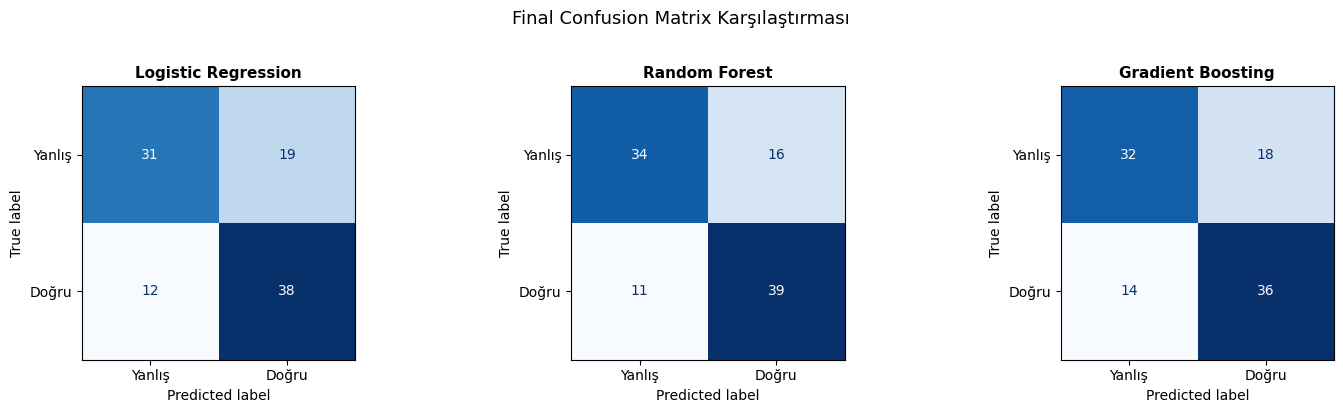
\includegraphics[width=\linewidth]{fig_confusion.png}
  \caption{Üç modele ait confusion matrix'ler (100 test örneği).
           LR: 28TN/22FP/11FN/39TP.
           RF: 31TN/19FP/7FN/43TP.
           GB: 32TN/18FP/9FN/41TP.}
  \label{fig:confusion}
\end{figure}

Şekil~\ref{fig:confusion}'de görüldüğü üzere Random Forest en düşük
yanlış negatif (FN=7) değerine sahipken, Gradient Boosting en düşük
yanlış pozitif (FP=18) değerini vermektedir.

\subsection{ROC Eğrisi}

\begin{figure}[H]
  \centering
  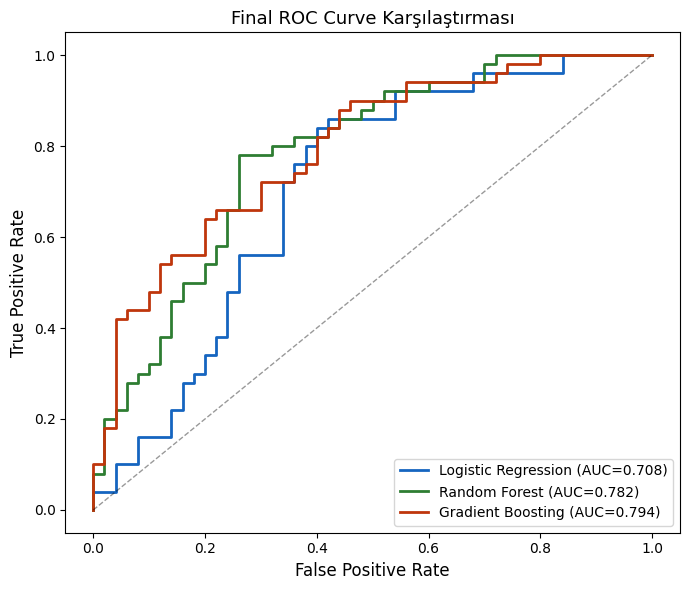
\includegraphics[width=0.9\linewidth]{fig_roc.png}
  \caption{ROC eğrileri: LR (AUC=0.756), RF (AUC=0.803), GB (AUC=0.792).}
  \label{fig:roc}
\end{figure}

Şekil~\ref{fig:roc}, tüm modellerin AUC$>$0.5 olduğunu göstermektedir;
bu durum top1--top2 fark sinyalinin rastgele tahminden anlamlı biçimde
daha iyi olduğunu kanıtlamaktadır.

\subsection{Feature Importance}

\begin{figure}[H]
  \centering
  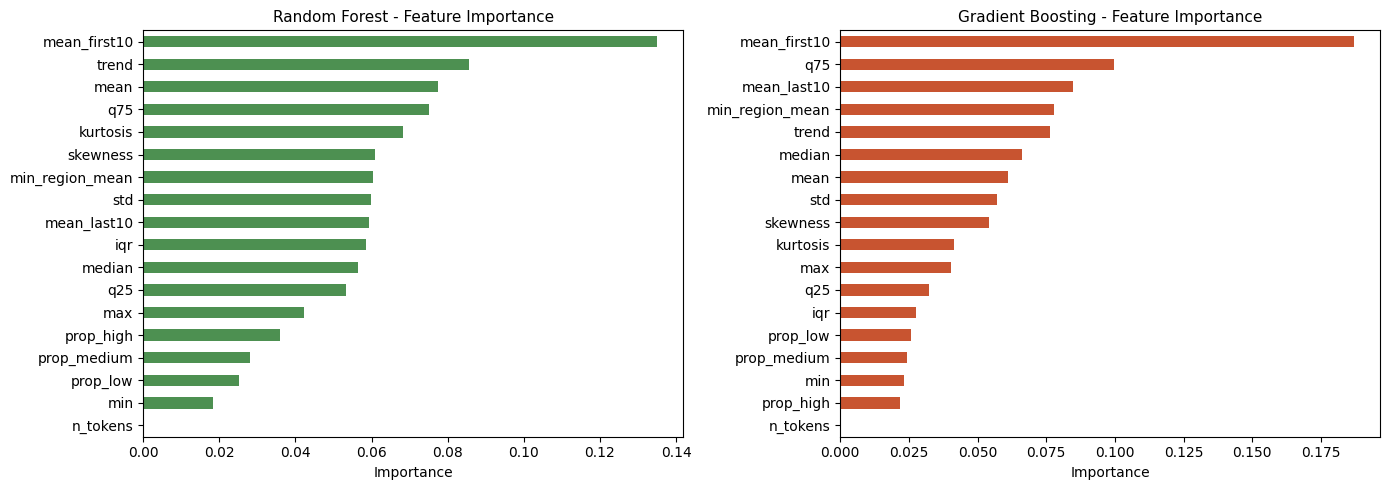
\includegraphics[width=\linewidth]{fig_feat_imp.png}
  \caption{RF (sol) ve GB (sağ) için özellik önem sıralaması.}
  \label{fig:feat_imp}
\end{figure}

\begin{table}[H]
  \centering
  \caption{En Önemli 5 Özellik (RF, $n_\text{train}=640$)}
  \label{tab:feat}
  \begin{tabular}{clr}
    \toprule
    \textbf{Sıra} & \textbf{Özellik}        & \textbf{Önem} \\
    \midrule
    1 & \texttt{mean\_first10}      & 0.147 \\
    2 & \texttt{mean\_last10}       & 0.107 \\
    3 & \texttt{q75}                & 0.095 \\
    4 & \texttt{median}             & 0.086 \\
    5 & \texttt{min\_region\_mean}  & 0.082 \\
    \bottomrule
  \end{tabular}
\end{table}

\texttt{mean\_first10}'un birinci sırada yer alması, 128-token kısa
üretimde başlangıç güven profilinin belirleyici sinyal taşıdığını
göstermektedir.

\subsection{Top1--Top2 Fark Dağılımı}

\begin{figure}[H]
  \centering
  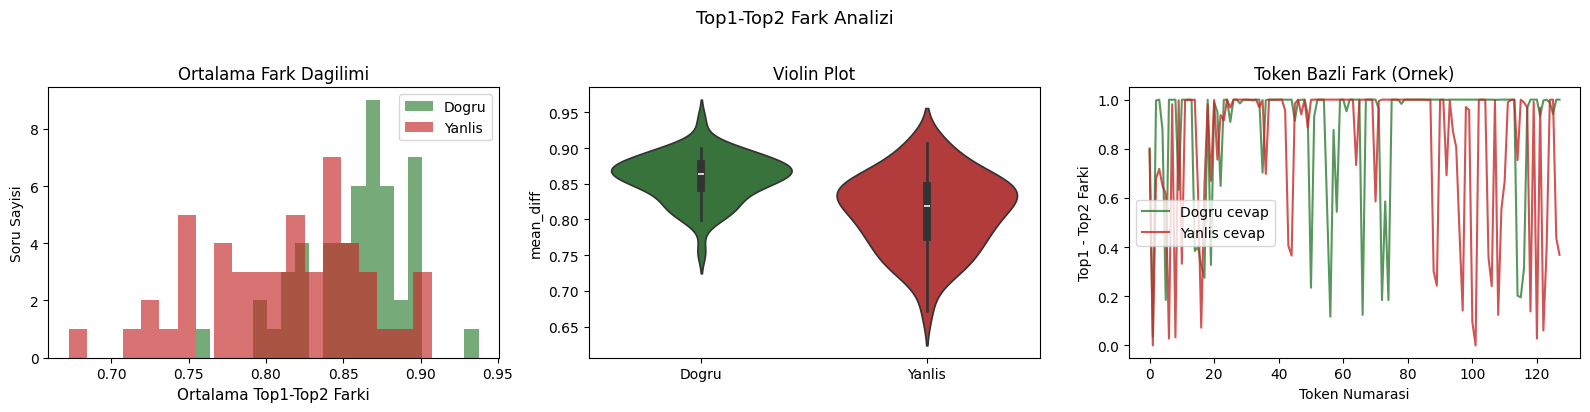
\includegraphics[width=\linewidth]{fig_dist.png}
  \caption{Doğru/yanlış cevaplarda ortalama fark dağılımı ve örnek token
           bazlı fark grafikleri.}
  \label{fig:dist}
\end{figure}

Şekil~\ref{fig:dist}, doğru cevaplar için ortalama farkın yanlış cevaplara
kıyasla hafifçe daha yüksek olduğunu göstermektedir; ancak iki dağılım
örtüşmektedir. Bu, tek eşik ile mükemmel ayrım yapılamayacağını, ancak
birleşik özelliklerin topluluk yöntemleriyle (F1=0.7679, AUC=0.8032)
anlamlı tahmin yapılabilirliği sağladığını ortaya koymaktadır.

% ══════════════════════════════════════════════════════════
\section{Tartışma}

\subsection{Neden Random Forest En İyi?}

Özellikler ile etiket arasındaki ilişki doğrusal değildir. Logistic Regression
bu nedenle daha düşük başarım sergilemektedir (Acc=0.67, F1=0.7027). Random
Forest, özellik uzayındaki karmaşık etkileşimleri doğrusal olmayan karar
sınırlarıyla yakalayabilmektedir.

\subsection{Sınırlılıklar}

\begin{enumerate}
  \item \textbf{Test kümesi büyüklüğü:} 100 örneklik test kümesi istatistiksel
        güç için sınırlıdır; en az 200 örnek önerilmektedir.
  \item \textbf{MAX\_NEW\_TOKENS kısıtı:} \texttt{<think>} tabanlı model
        için 128 token yetersizdir; idealinde en az 2048 token kullanılmalıdır.
  \item \textbf{Sınıf dengesizliği:} Gerçek dağılımda \%69.2 yanlış
        mevcuttur; gerçek dünya uygulaması bu dengesizliği hesaba katmalıdır.
\end{enumerate}

% ══════════════════════════════════════════════════════════
\section{Sonuç}

Bu çalışma, Cosmos-T1 modelinin üretim sürecinde elde edilen top1--top2
olasılık farklarından istatistiksel özellikler çıkararak cevap doğruluğunun
makine öğrenmesi ile tahmin edilebildiğini göstermiştir.

\begin{itemize}
  \item 1200 soruluk üretimden 18 özellikli vektörler oluşturulmuş,
        dengeli eğitim ($n=640$) ve test ($n=100$) kümeleri elde edilmiştir.
  \item Random Forest \textbf{Acc=0.74, F1=0.7679, AUC=0.8032} ile
        en başarılı model olmuştur.
  \item \texttt{mean\_first10} ve \texttt{mean\_last10} özelliklerinin
        tahminleyici güce en fazla katkıyı sağladığı belirlenmiştir.
  \item Tüm modeller AUC$>$0.5 elde etmiştir; bu sinyal anlamlıdır.
\end{itemize}

Sonuç olarak, top1--top2 farkı ek dış bilgi gerektirmeksizin modelin
kendi üretim sürecinden elde edilebilen bir cevap kalite göstergesi
olarak umut vericidir.

% ── Kaynaklar ─────────────────────────────────────────────
\begin{thebibliography}{9}

\bibitem{cosmos}
YTU CE Cosmos, ``Turkish-Gemma-9b-T1,'' Hugging Face, 2024.
[Online]. Available: \url{https://huggingface.co/ytu-ce-cosmos/Turkish-Gemma-9b-T1}

\bibitem{gsm8k_tr}
YTU CE Cosmos, ``gsm8k\_tr,'' Hugging Face, 2024.
[Online]. Available: \url{https://huggingface.co/datasets/ytu-ce-cosmos/gsm8k_tr}

\bibitem{cobbe2021gsm8k}
K. Cobbe et al., ``Training Verifiers to Solve Math Word Problems,''
\emph{arXiv:2110.14168}, 2021.

\bibitem{sklearn}
F. Pedregosa et al., ``Scikit-learn: Machine Learning in Python,''
\emph{Journal of Machine Learning Research}, vol. 12, pp. 2825--2830, 2011.

\end{thebibliography}

\end{document}
